\chapter{Polarimetría}

Esta clase tiene como objetivo comprender los conceptos básicos de polarimetria. Para ello veremos como obtener las matrices polarimétricas y generar a partir de ellas distintas descomposiciones que nos den información sobre el blanco.

\section{Calculo de matrices polarimétricas}

Para poder realizar descomposiciones polatrimétricas es necesario conservar la información completa de la imagen SAR a lo largo de todo el proceso. Para hacer esto repetiremos los pasos vistos en la clase anterior, pero haciendo foco en como mantener dicha información.

\subsection{Calibración}
Abra la imagen \directory{ALPSRP278916070-L1.1.zip} que descargo del Alaska Satellite Facility.  Dirijase al menu \menu{Radar>Radiometric>Calibrate} (Figura \ref{fig:calibrar}). En este caso, tilde la opción \emph{Save as complex output} en \emph{Processing parameters}

\begin{figure}[h!]
    \centering
    \subfloat[I/O Parameters]{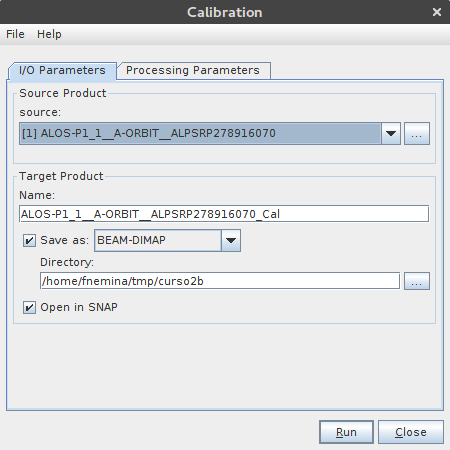
\includegraphics[width=0.35\textwidth]{fig:calibrar1.png}}
    \hfill
    \subfloat[Processing parameters]{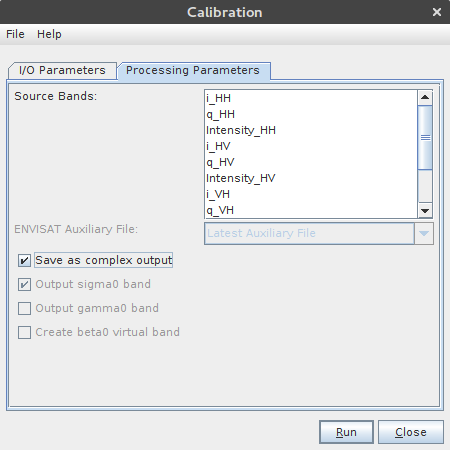
\includegraphics[width=0.35\textwidth]{fig:calibrar3.png}}
    \caption{}
    \label{fig:calibrar}
\end{figure}

\subsection{Calculo de matriz de coherencia}

Para calcular la matriz de coherencia, una vez calibrada la imagen utilice la herramienta \menu{Radar>Polarimetric>Polarimetric matrix generation}.

Seleccione la imagen \directory{ALOS-P1\_1\_\_A-ORBIT\_\_ALPSRP278916070\_Cal} y en Processing parameters elija la matrix T3. No se preocupe por el significado de esta matriz actualmente (Figura \ref{fig:t3}).

\begin{figure}[h!]
    \centering
    \subfloat[I/O Parameters]{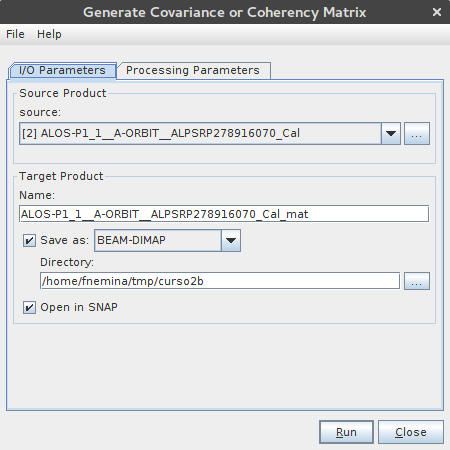
\includegraphics[width=0.35\textwidth]{fig:t31.png}}
    \hfill
    \subfloat[Processing parameters]{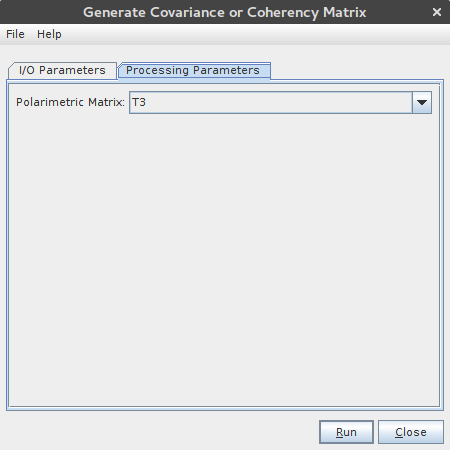
\includegraphics[width=0.35\textwidth]{fig:t32.png}}
    \caption{}
    \label{fig:t3}
\end{figure}

\subsection{Filtrado}

En el caso de imagenes full polarimetricas existen distintos tipos de filtros para aplicar. Para usarlos vaya al menu \menu{Radar>Polarimetric>Polarimetric speckle filter}. Utilice en este caso el filtro \menu{Refined Lee} sobre la imagen \directory{ALOS-P1\_1\_\_A-ORBIT\_\_ALPSRP278916070\_Cal\_mat} (Figura \ref{fig:plee})

\begin{figure}[h!]
    \centering
    \subfloat[I/O Parameters]{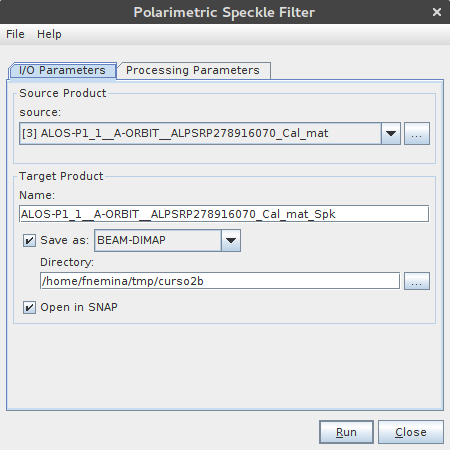
\includegraphics[width=0.35\textwidth]{fig:plee1.png}}
    \hfill
    \subfloat[Processing parameters]{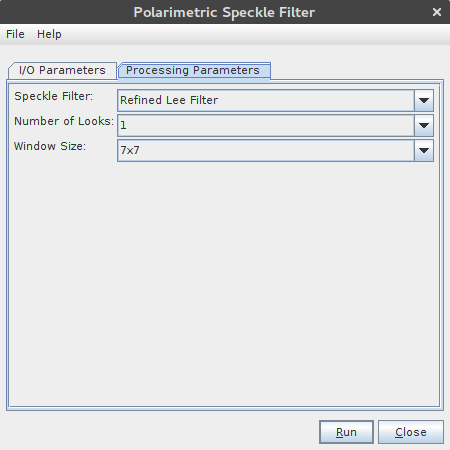
\includegraphics[width=0.35\textwidth]{fig:plee2.png}}
    \caption{}
    \label{fig:plee}
\end{figure}

\subsection{Proyección}

Puede ahora reproyectar la imagen en el terreno aplicando los procesos de \emph{Deskewing} y proyección sobre un modelo de elevación digital.

\section{Descomposición de Pauli}

La descomposición de Pauli nos permite en una imagen full polarimétrica separar la información sobre interacciones de tipo doble rebote, en volumen y especulares.

La descomposición general da tres canales que suelen interpretarse de la siguiente manera:

\begin{itemize}
    \item Rojo: Información por procesos de un solo rebote o un número impar par de rebotes.
    \item Verde: Información por procesos de scatering en volumen.
    \item Azul: Información por procesos de doble rebote o un número par de rebotes.
\end{itemize}

Obtenga la descomposición de Pauli usando la herramienta \menu{Radar>Polarimetric>Polarimetric Decomposition} seleccionando como imagen de entrada la corregida en terreno y como descomposición la de Pauli (Figura \ref{fig:pauli})

\begin{figure}[h!]
    \centering
    \subfloat[I/O Parameters]{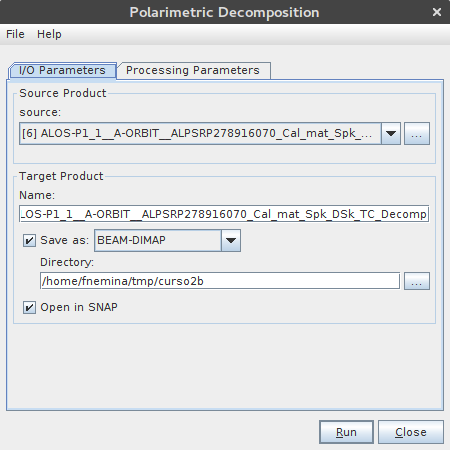
\includegraphics[width=0.35\textwidth]{fig:pauli1.png}}
    \hfill
    \subfloat[Processing parameters]{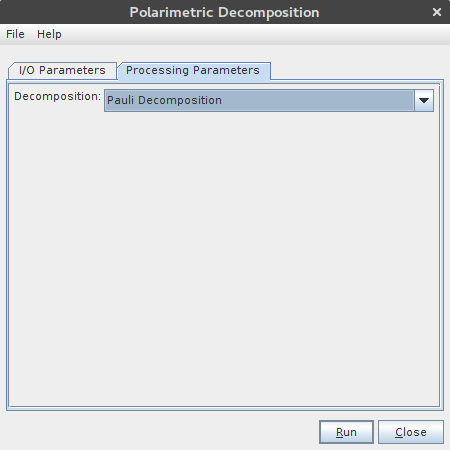
\includegraphics[width=0.35\textwidth]{fig:pauli2.png}}
    \caption{}
    \label{fig:pauli}
\end{figure}

Observe la descomposición de Pauli haciendo click derecho sobre la imagen obtenida y seleccionando la opción \emph{Open RGB image window} (Figura \ref{fig:pauli}).

\begin{figure}[h!]
    \centering
    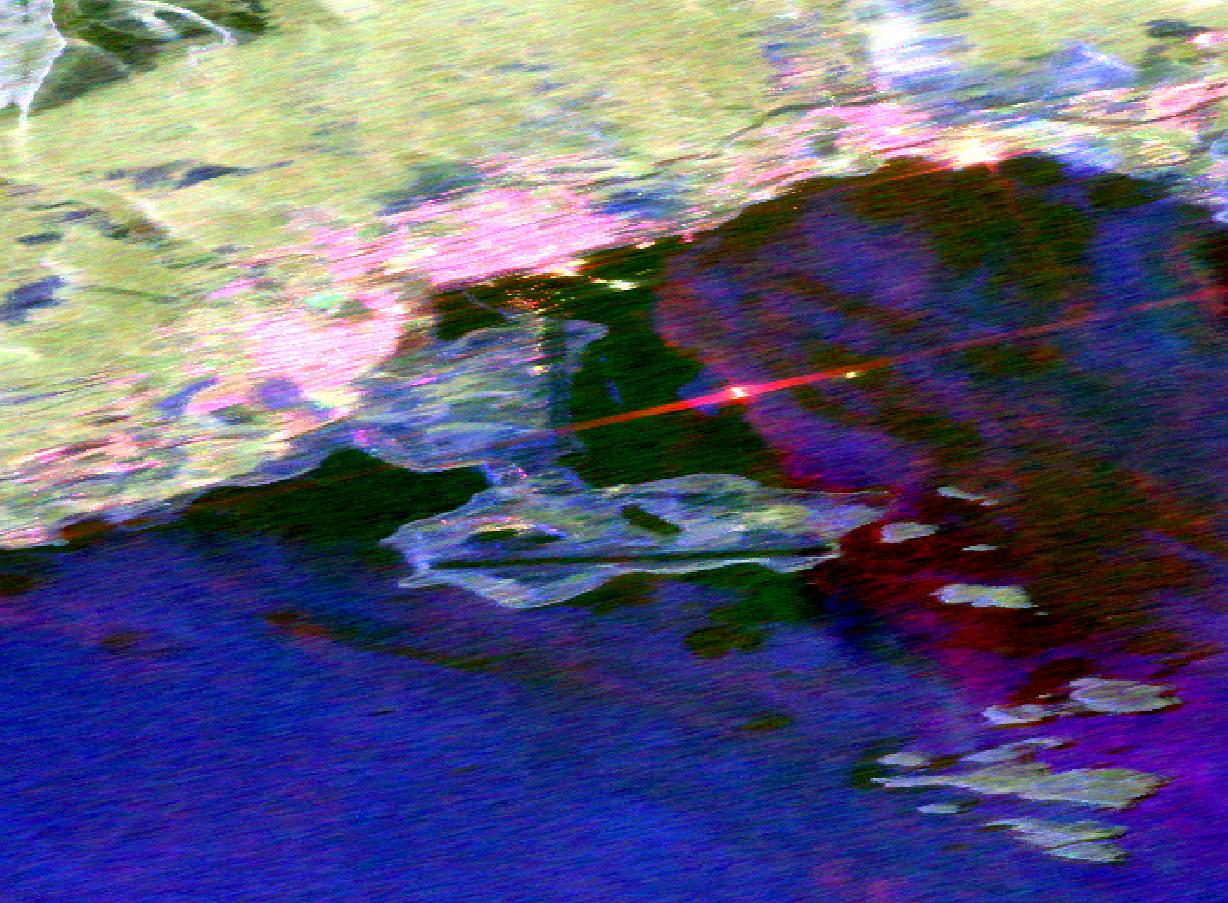
\includegraphics[width=0.7\textwidth]{fig:pauli.jpg}
    \caption{}
    \label{fig:pauli}
\end{figure}

\section{Actividades}

\begin{que}
    ¿De que color se ven las zonas urbanas en la descomposición de Pauli?
\end{que}

\begin{que}
    ¿De que color se ven los bosques en la descomposición de Pauli?
\end{que}

\begin{que}
    ¿De que color se ve el agua en la descomposición de Pauli?
\end{que}

\begin{que}
    ¿De que color se ve la pista de aterrizaje en la descomposición de Pauli?
\end{que}
